\documentclass[9pt,twocolumn]{article}
\usepackage[margin=0.62in]{geometry}
\usepackage[T1]{fontenc}
\usepackage{lmodern,microtype}
\usepackage{graphicx,booktabs,tabularx,xcolor,hyperref,tikz}
\usetikzlibrary{arrows.meta,positioning,shapes.geometric,fit}
\hypersetup{colorlinks=true,linkcolor=teal,urlcolor=teal,citecolor=teal}
\setlength{\columnsep}{0.24in}
\title{Vascularis AI: Leakage-Aware Prediction and Interactive Coronary Risk Visualization}
\author{Hackathon Track A Technical Report}
\date{October 2026}
\begin{document}\maketitle
\begin{abstract}
We present Vascularis AI, a web prototype that combines tabular prediction of coronary artery disease (CAD) and vessel stenosis with an interactive 3D heart visualization. Experiments use the 303-record Extension of Z-Alizadeh Sani dataset. Angiography-derived targets (Cath, LAD, LCX, RCA) are excluded from every model input. On a shared 10-fold CAD split, TabPFN obtains 88.12\% accuracy (AUC 0.9352), versus 85.81\% (AUC 0.9299) for logistic regression. TabPFN has the strongest measured LAD and RCA accuracies (79.87\% and 67.33\%); CatBoost leads LCX (70.30\%). Experimental winners are distinguished from the saved pipelines serving the application. These are internal estimates on a small dataset, not clinical validation.
\end{abstract}
\noindent\textbf{Keywords:} coronary artery disease, TabPFN, tabular learning, leakage prevention, visualization
\section{Introduction}
CAD is associated with narrowing of one or more coronary arteries. Track A asks for CAD and LAD/LCX/RCA prediction, interactive vessel-specific 3D mapping, an explanation dashboard, and an explicit clinical safety disclaimer. Vascularis addresses these requirements through a React web experience, a prediction API, and serialized scikit-learn/CatBoost/TabPFN-derived artifacts. Since the source dataset is small, we prioritize leakage control and transparent limits over headline accuracy claims.
\section{Data and methods}
\subsection{Dataset and target isolation}
The UCI Extension of Z-Alizadeh Sani workbook contains 303 patient records and demographic, examination, ECG, laboratory, and echocardiographic variables. CAD is represented by Cath; vessel endpoints are LAD, LCX, and RCA. For every endpoint all four angiographic columns are removed from the predictors, preventing direct label leakage between related targets. Mixed categorical and numeric inputs are imputed and encoded within training partitions.
\subsection{Models and validation}
We evaluated class-weighted logistic regression, CatBoost, a heterogeneous stack, a 17-feature genetic feature-selection stack, and TabPFN (a pretrained transformer for small tabular data). The common vessel comparison uses shuffled stratified 10-fold CV (seed 42), with threshold 0.5. The genetic selector is rerun within each training fold; the TabPFN encoder is fitted on each training fold. CAD TabPFN/logistic scores are also from shared shuffled stratified 10-fold splits. Reported accuracy is the fraction of correct predictions; ROC-AUC uses held-out probabilities. Results across distinct protocols are not directly comparable.
\begin{figure*}[t]\centering
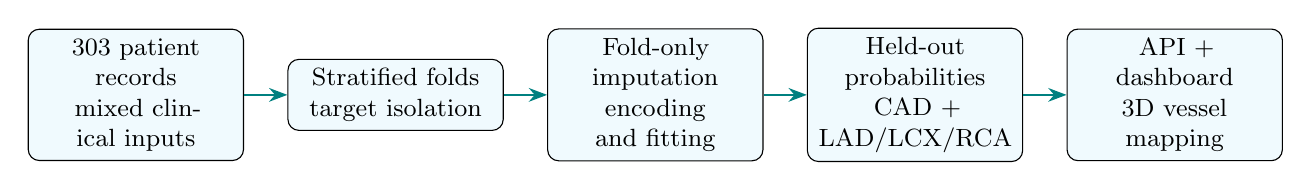
\begin{tikzpicture}[node distance=0.45cm and 0.55cm, box/.style={draw,rounded corners,fill=cyan!6,align=center,minimum height=0.65cm,text width=2.5cm,font=\small}, arr/.style={-{Stealth},thick,teal}]
\node[box] (data) {303 patient records\\mixed clinical inputs};
\node[box,right=of data] (split) {Stratified folds\\target isolation};
\node[box,right=of split] (fit) {Fold-only imputation\\encoding and fitting};
\node[box,right=of fit] (predict) {Held-out probabilities\\CAD + LAD/LCX/RCA};
\node[box,right=of predict] (ui) {API + dashboard\\3D vessel mapping};
\draw[arr](data)--(split);\draw[arr](split)--(fit);\draw[arr](fit)--(predict);\draw[arr](predict)--(ui);
\end{tikzpicture}
\caption{Prediction and visualization pipeline. The four angiography-derived target columns are never model inputs.}
\end{figure*}
\subsection{Application and interpretation}
The browser exposes all 55 clinical predictors through basic and expanded forms, displays four probabilities and CAD classification at threshold 0.5, and colors three selectable vessel locator nodes. Three.js loads a locally hosted textured GLB cutaway with orbit, zoom, touch and reset controls. The CC0 Grab3D asset discloses AI-assisted generation: it is an educational illustration, not medically validated anatomy. Node locations are schematic rather than lesion coordinates; expert anatomical review is still needed. The API provides health/schema/prediction routes and explicit missing-field disclosure. A fixed robot guide assists users without exposing backend architecture names.

The serving CAD pipeline is logistic regression; LAD/RCA use saved probability blends and LCX uses CatBoost. Their stored five-fold accuracies are 87.13\%, 79.54\%, 67.66\%, and 68.98\% for CAD/LAD/LCX/RCA respectively. These serving results must not be confused with the ten-fold experimental comparison below. For CAD, the dashboard computes exact additive evidence relative to a cohort reference: $\Delta_j=\beta_j(z_j-z_j^{\rm ref})$. Encoded contributions are grouped by original feature. The reference log-odds plus the sum of contributions reconstructs the current prediction. Actual input values and direction of influence are shown; this explanation is associative, not causal, and is not SHAP. Vessel-level explanations remain future work. The UI retains the required educational decision-support disclaimer.
\begin{figure}[t]\centering
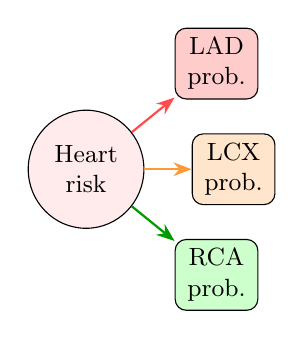
\begin{tikzpicture}[node distance=0.35cm, vessel/.style={draw,rounded corners,align=center,minimum width=1.05cm,minimum height=.48cm,font=\small}, heart/.style={draw,ellipse,fill=red!8,minimum width=1.25cm,minimum height=1.5cm,align=center,font=\small}, arr/.style={-{Stealth},thick}]
\node[heart] (h) {Heart\\risk};
\node[vessel,above right=0.35cm and 0.6cm of h,fill=red!20] (lad) {LAD\\prob.};
\node[vessel,right=0.6cm of h,fill=orange!20] (lcx) {LCX\\prob.};
\node[vessel,below right=0.35cm and 0.6cm of h,fill=green!20] (rca) {RCA\\prob.};
\draw[arr,red!70](h)--(lad);\draw[arr,orange!80](h)--(lcx);\draw[arr,green!60!black](h)--(rca);
\end{tikzpicture}
\caption{Conceptual vessel-risk overlay: colors encode predicted probability, not measured lesion geometry.}
\end{figure}
\section{Results}
\begin{table}[h]\centering\small\caption{CAD, common 10-fold evaluation}\begin{tabular}{lrrr}\toprule Model&Acc.&F1&AUC\\\midrule Logistic regression&85.81&0.8969&0.9299\\TabPFN&\textbf{88.12}&\textbf{0.9178}&\textbf{0.9352}\\Paper-style SVM reproduction&84.16&0.8947&0.9000\\\bottomrule\end{tabular}\end{table}
\begin{table}[h]\centering\small\caption{Vessel accuracy, shared 10-fold split}\begin{tabular}{lrrr}\toprule Target&CatBoost&GA stack&TabPFN\\\midrule LAD&75.25&75.58&\textbf{79.87}\\LCX&\textbf{70.30}&62.38&66.67\\RCA&64.69&66.34&\textbf{67.33}\\\bottomrule\end{tabular}\end{table}
TabPFN improves CAD accuracy by 2.31 percentage points over logistic regression on the shared split. Vessel AUCs for TabPFN are 0.8443 (LAD), 0.7263 (LCX), and 0.7293 (RCA). Published vessel results of 89.68\%, 88.71\%, and 85.81\% are higher; our same-fold comparison does not beat those figures. The separate CAD paper reports 97.67\%; our comparison against a paper-style approximation also does not reproduce or exceed that headline. Differences in implementation and unspecified search details limit equivalence.
\section{Discussion and limitations}
TabPFN is a useful pretrained baseline on this small tabular dataset, but the gains are modest and based on one split scheme. The vessel genetic-stack comparison results from an approximate implementation of the published method, not an exact replication. No independent test cohort is available; fold estimates can vary substantially with 303 records. Inputs may be incomplete, the study population may not represent deployment users, and anatomical coloring indicates model probability rather than observed lesion location. Future work should prioritize external/multicenter validation, confidence intervals, calibration, subgroup checks, and clinician review. More elaborate neural networks or reinforcement learning are not justified by this static, small supervised dataset.
\section{Conclusion}
Vascularis delivers the requested prototype architecture and a transparent evaluation trail. TabPFN currently leads our measured CAD and LAD accuracy; CatBoost leads LCX and TabPFN marginally leads RCA. We do not claim to exceed published benchmarks. Responsible progress requires a larger independent dataset and exact, preregistered protocol reproduction.
\section*{Reproducibility and safety}
Scripts and JSON metrics are in \texttt{ml/} and \texttt{reports/}. The source workbook is under \texttt{data/raw/uci\_411/}. Local TabPFN inference requires accepting the relevant Prior Labs license and setting \texttt{TABPFN\_TOKEN}; never commit credentials. This prototype is not for diagnosis, triage, or treatment decisions.
\begin{thebibliography}{9}\small
\bibitem{uci} UCI Machine Learning Repository. Extension of Z-Alizadeh Sani Dataset, dataset 411. \url{https://archive.ics.uci.edu/dataset/411/extension+of+z-alizadeh+sani}.
\bibitem{tabpfn} Hollmann et al. TabPFN: A Transformer That Solves Small Tabular Classification Problems in a Second. Nature, 2025. \url{https://www.nature.com/articles/s41586-024-08328-6}.
\bibitem{track} Multimodal AI Hackathon 2026. Track A: Cardiovascular Risk Visualization \& Prediction. Project brief.
\end{thebibliography}
\end{document}
